\section{An infinite quotient compatible with the family}
\label{sec:quotient}

We now impose the geometric relations. The order of the choices matters. We first make the parameter monodromy sufficiently deep, then compactify the resulting finite cover of the marked family, and only then choose powers for its finitely many remaining boundary meridians.

\subsection{All deep monodromies from a controlled set of relations}

Write $\widehat\Gamma$ for the free pro-2 completion of the rank-four parameter group $\Gamma$. Give its four free generators ordinary Magnus degree one, and let
\[
 D_N=\{m\in\widehat\Gamma:\nu_\Gamma(m)\ge N\},
 \qquad \Gamma_N=\Gamma\cap D_N.
\]
Each $D_N$ is open and normal, and these subgroups form a neighborhood basis of the identity. The leading degree-$N$ Magnus part embeds
\[
 D_N/D_{N+1}\hookrightarrow
 \F_2\{\text{words of length }N\text{ on four letters}\}.
\]
In particular, its dimension is at most $4^N$. Choose a set $\mathcal M_N\subset\Gamma_N$ representing a basis of this quotient. Discrete representatives exist by density and openness. For any integer $J\ge1$, the union of the $\mathcal M_N$, $N\ge J$, topologically generates $D_J$: successive removal of the leading part approximates every element modulo each $D_N$.

By \Cref{prop:monodromy-raising}, the automorphisms associated with the four generators of $\Gamma$ differ from the identity by operators raising degree on the Magnus algebra of $\widehat F$. Substitute these four operators into the base Magnus expansion, as in \Cref{lem:substitution}. It follows that the action extends continuously to $\widehat\Gamma$ and that
\begin{equation}\label{eq:deep-action}
 (\varphi_m-\id)(A_{F,\ge d})\subset A_{F,\ge d+N}
 \qquad(m\in D_N).
\end{equation}
Indeed, on each finite truncation these actions lie in a finite unipotent 2-group, so completion introduces no extra continuity assumption. The action preserves $\widehat K$, since the actual action on the closed torus is $\pm\id$ and preserves reduction modulo four.

Recall that $K$ is free of rank $97$. Fix a free basis $k_1,\ldots,k_{97}$. By the completion identification in \Cref{sec:transfer}, this is a topological generating set of $\widehat K$.

We count monodromies by their depth in the filtration. This lets us
control the relation cost without estimating the free rank of the
finite-index subgroup $\Gamma_J$. The
bound $4^N$ will be offset by the higher degree $N+1$ of the resulting
fiber relations.

For every $N\ge J$, $m\in\mathcal M_N$ and $1\le i\le97$, impose on $L$ the relator
\begin{equation}\label{eq:monodromy-relators}
 \Phi\bigl(\varphi_m(k_i)k_i^{-1}\bigr).
\end{equation}
Its argument belongs to $\widehat K$ and has $F$-degree at least $N+1$ by \eqref{eq:deep-action}. Its $L$-degree is at least $N+1$ by \Cref{lem:transfer}. Thus these relators have total cost at most
\begin{equation}\label{eq:monodromy-cost}
 97\sum_{N\ge J}4^N t^{N+1}
 =97t\frac{(4t)^J}{1-4t},\qquad 0<t<\frac14.
\end{equation}

Let $Q_0$ be the quotient of $L$ by the closed normal subgroup generated by these relators and the $24$ involution relators of \Cref{prop:involution}. The following observation is what turns the counted relations into \emph{all} the required equalities.

\begin{lemma}\label{lem:deep-invariance}
The homomorphism $f_K:\widehat K\to Q_0$ induced by $\Phi$ satisfies
\[
 f_K\varphi_m=f_K\qquad(m\in D_J).
\]
Consequently the induced homomorphism $\Pi\to Q_0$ from the punctured sphere is invariant under its actual based monodromy for every $m\in\Gamma_J$.
\end{lemma}

\begin{proof}
For each imposed $m$, equality on the basis $k_i$ gives equality of the two continuous homomorphisms on all of $\widehat K$. The set
\[
 E_0=\{m\in\widehat\Gamma:f_K\varphi_m=f_K
                     \text{ on }\widehat K\}
\]
is a closed subgroup. For multiplication, apply one equality to $\varphi_n(k)$ and then the other to $k$; for inverses apply the equality to $\varphi_m^{-1}(k)$. Closedness follows from continuity. It contains all $\mathcal M_N$ with $N\ge J$, and hence contains $D_J$.

The last assertion uses the actual surjection $K\to\Pi$ and its exact compatibility with the two based actions, proved in \Cref{prop:based-monodromy,lem:pinched-sphere}. Surjectivity onto the unpinched sphere group is essential here; no invariance of the pinching kernel was assumed in defining the relators.
\end{proof}

\subsection{A finite parameter cover with ramification index two}

The monodromy series in \eqref{eq:monodromy-cost} requires $4t<1$.
The involution leaves the weighted expression $1-G(t)$, where
$G(t)=3t(1+t)(1+t^2)^2$, so we also need $G(t)>1$.
Both conditions hold for $t$ sufficiently close to $1/4$ from below.
We choose the following rational value and check its exact margin
in \Cref{prop:infinite-quotient}:
\begin{equation}\label{eq:t-choice}
 t=\frac{49}{200}<\frac14.
\end{equation}
We reserve $1/100$ of the relation bound for deep monodromy and another
$1/100$ for the final boundary powers; the strict inequality below will
justify both allowances. Choose $J$ large enough that \eqref{eq:monodromy-cost} is less than $1/100$. Enlarge $J$, if necessary, until $\Gamma_J$ kills the finite permutation and sign action of \Cref{lem:finite-geometric-monodromy}. This is possible because that action has finite 2-group image.

Set
\[
 M=\langle\gamma_*^2\rangle\Gamma_J\subset\Gamma.
\]
Normality of $\Gamma_J$ makes this a finite-index subgroup. The action of $\gamma_*^2$ on the pinched sphere group is trivial, by \Cref{lem:finite-geometric-monodromy}. Together with \Cref{lem:deep-invariance}, this proves invariance of $\Pi\to Q_0$ under all of $M$. Moreover $M$ fixes every marking and lies in the parameter sign kernel. It contains $\gamma_*^2$ but not $\gamma_*$.

Let $B'\to B$ be the connected finite cover corresponding to $M$, and let $C'$ be its smooth projective completion. These are algebraic: Riemann existence applies to finite covers of a complex variety without a properness hypothesis \citep[Expos\'e XII, Th\'eor\`eme 5.1]{SGA1}, and normalization compactifies the curve cover. The selected point $c_*\in C'\setminus B'$ has ramification index exactly two over $s_*$, since $\langle\gamma_*\rangle\cap M=\langle\gamma_*^2\rangle$.

The $48$ markings split into disjoint algebraic sections over $B'$. Denote their complement by
\[
 U\subset\PP^1\times B'.
\]
Finite-point isotopy gives a locally trivial punctured-sphere bundle. The open base curve is aspherical, and the fixed section at $q(0)$ splits its fundamental-group sequence. Therefore
\[
 \pi_1(U)=\Pi\rtimes M.
\]
The monodromy invariance just proved extends $\Pi\to Q_0$ to a homomorphism
\begin{equation}\label{eq:rho-zero}
 \rho_0:\pi_1(U)\longrightarrow Q_0
\end{equation}
that kills the section subgroup $M$. Its restriction to every punctured fiber has dense image, because the pinched sphere group maps densely onto the pro-2 quotient $Q_0$.

\subsection{Separating the sections and filling the distinguished fiber}

Extend the marked sections across $C'\setminus B'$ in $\PP^1\times C'$. Blow up their collision points until their strict transforms are disjoint, obtaining a smooth projective surface
\[
 Y\longrightarrow C'
\]
with $U$ unchanged. This terminates: at any common point of two sections, a blowup decreases their intersection multiplicity by one, so the sum of all pairwise intersection multiplicities strictly decreases.

All fibers over $C'\setminus B'$ stay reduced with simple normal crossings. Here is the local induction, which also ensures that the full boundary is a simple normal crossing divisor. At a smooth point of a reduced vertical component, take the projection coordinate $u$ and write a section as $w=g(u)$. Blowing up the origin gives the chart $w=uv$, where the transformed section is $v=g(u)/u$ and is still transverse to the new multiplicity-one component $u=0$. In the other chart the projection has the form $u=wb$; its differential vanishes at the vertical node $w=b=0$. A section cannot pass through that node, because its composite with the projection is the identity. Thus every further collision center is a smooth point of a reduced vertical component. When the sections are disjoint, each meets a single vertical component transversely and avoids all vertical nodes. The boundary
\[
 D=Y\setminus U
\]
is consequently a simple normal crossing divisor: locally it is defined
by $u=0$ or $uv=0$ in smooth coordinates. It contains the $48$
horizontal marked sections and every component of the fibers over
$C'\setminus B'$.

Over $c_*$ the local marking equation is $w^2=s-s_*$. After the base change of index two it becomes $w^2=u^2$, up to analytic coordinate changes. One blowup separates the two branches $w=\pm u$. Hence the distinguished fiber $D_*$ consists of one main sphere and $24$ tails. Every tail carries two marked sections and meets the main sphere once; the main sphere carries none.

\begin{figure}[htbp]
\centering
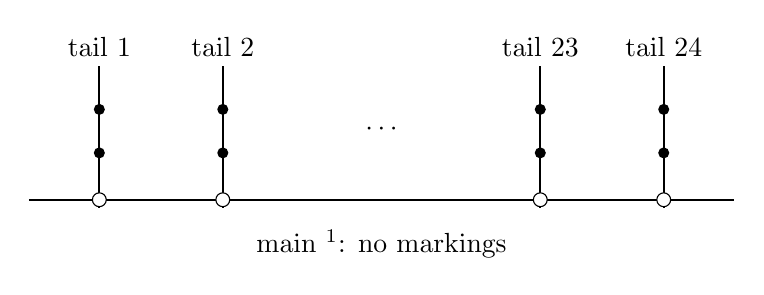
\begin{tikzpicture}[x=1.12cm,y=0.85cm]
 \draw[thick] (0,0) -- (8,0);
 \foreach \x/\lab in {0.8/1,2.2/2,5.8/23,7.2/24} {
  \draw[thick] (\x,-0.12) -- (\x,2);
  \draw[fill=white] (\x,0) circle (2.5pt);
  \fill (\x,0.7) circle (2pt);
  \fill (\x,1.35) circle (2pt);
  \node[above] at (\x,2) {tail $\lab$};
 }
 \node at (4,1.05) {$\cdots$};
 \node[below] at (4,-0.3) {main $\PP^1$: no markings};
\end{tikzpicture}
\caption{The distinguished fiber $D_*$ on $Y$, after the base change of index two and
one blowup at each collision. Each of the $24$ rational tails has two
markings (solid dots) and one node on the main component (open circles).
The middle $20$ tails are omitted. The cover constructed in \Cref{sec:surface}
is unramified at the nodes and can branch only at the markings. Its
inverse image may have a different incidence graph.}
\label{fig:distinguished-fiber}
\end{figure}


\begin{lemma}\label{lem:distinguished-meridians}
Every meridian around a component of $D_*$ has trivial image under $\rho_0$.
\end{lemma}

\begin{proof}
A main-component meridian is represented by the circuit along the fixed exterior section, so it is killed by \eqref{eq:rho-zero}.

For a tail use the blowup chart $w=uv$. A meridian at a sufficiently large fixed slope $v=c$ is represented downstairs by
\[
 u=\varepsilon e^{i\theta},\qquad
 w=c\varepsilon e^{i\theta},\qquad 0\le\theta\le2\pi.
\]
Choose $|c|$ larger than the two branch slopes and then choose $\varepsilon$ small. Trivialize the pair motion by an isotopy supported inside the circle containing the two marks but not this meridian. In this trivialization the loop is the base circuit followed by one full pair-boundary loop, up to conjugacy and the choice of multiplication convention. The base circuit is killed by the section splitting; the pair boundary is killed by the pinching map. Both factors therefore have trivial image.
\end{proof}

\subsection{The remaining boundary relations}

There are finitely many components of $D$ outside $D_*$. Choose based meridians $\mu_1,\ldots,\mu_b$ for them, and choose lifts $\widetilde\mu_i\in L$ of $\rho_0(\mu_i)\in Q_0$. These lifts exist since $L\to Q_0$ is surjective. Choose an integer $e$ so large that
\begin{equation}\label{eq:boundary-cost}
 b\,t^{2^e}<\frac1{100},
\end{equation}
and impose the additional relators $\widetilde\mu_i^{2^e}$.
This is the high-power method underlying Golod's construction
\citep{Golod1964}, applied here to the finitely many boundary elements.
Each added relator has degree at least $2^e$ by
\eqref{eq:degree-rules}. Denote the resulting pro-2 quotient by $Q$.

\begin{proposition}\label{prop:infinite-quotient}
The group $Q$ is infinite. The homomorphism
\[
 \rho:\pi_1(U)\longrightarrow Q
\]
induced by $\rho_0$ has dense image on every punctured fiber. Each component meridian of $D$ has finite image, and every component meridian of $D_*$ has trivial image.
\end{proposition}

\begin{proof}
Only infinitude remains to prove. The generators of $L$ have polynomial $P(t)$ and the involution relators have cost at most $tG(t)$, where \Cref{prop:involution} gives
\[
 P(t)=(1+t)G(t),\qquad
 G(t)=3t(1+t)(1+t^2)^2.
\]
At the rational value \eqref{eq:t-choice}, $t^2>3/50$, so
\[
 G(t)>
 \frac{3\cdot49\cdot249\cdot53^2}{200^2\cdot50^2}
 =\frac{102817827}{100000000}
 >\frac{257}{250}.
\]
The complete weighted expression in \Cref{lem:weighted-gs} is therefore less than
\[
 1-P(t)+tG(t)+\frac1{100}+\frac1{100}
 =1-G(t)+\frac1{50}
 <-\frac1{125}<0.
\]
The infinite monodromy-relator family is finite in each bounded degree and has convergent cost by \eqref{eq:monodromy-cost}. The remaining families are finite. All hypotheses of \Cref{lem:weighted-gs} hold, proving that $Q$ is infinite. Passage to the quotient preserves all earlier equalities and the density of each fiber image.
\end{proof}

Notice that $e$ is chosen after the finite cover and compactification. Thus their possibly large number of boundary components introduces no circular parameter choice. The surface construction now uses only the finite local images and the infinite fiber image recorded in \Cref{prop:infinite-quotient}.
